%% fundamentals.tex
The biological neuronal system not only initially inspired neural networks but also this thesis.
Accordingly, in \secref{neurons}, it is explained how biological neurons work and they are related to their artificial counterparts.
Next, artificial neural networks, connecting many artificial neurons, are described in \secref{ann}.
In \secref{limitationsDL}, the limitations of such artificial neural networks are pointed out.
Finally, in \secref{neurocomputing}, biologically more plausible learning methods related to this thesis are explored.

\section{Human Brain}\seclbl{neurons}
\begin{figure}[h]
    \centering
    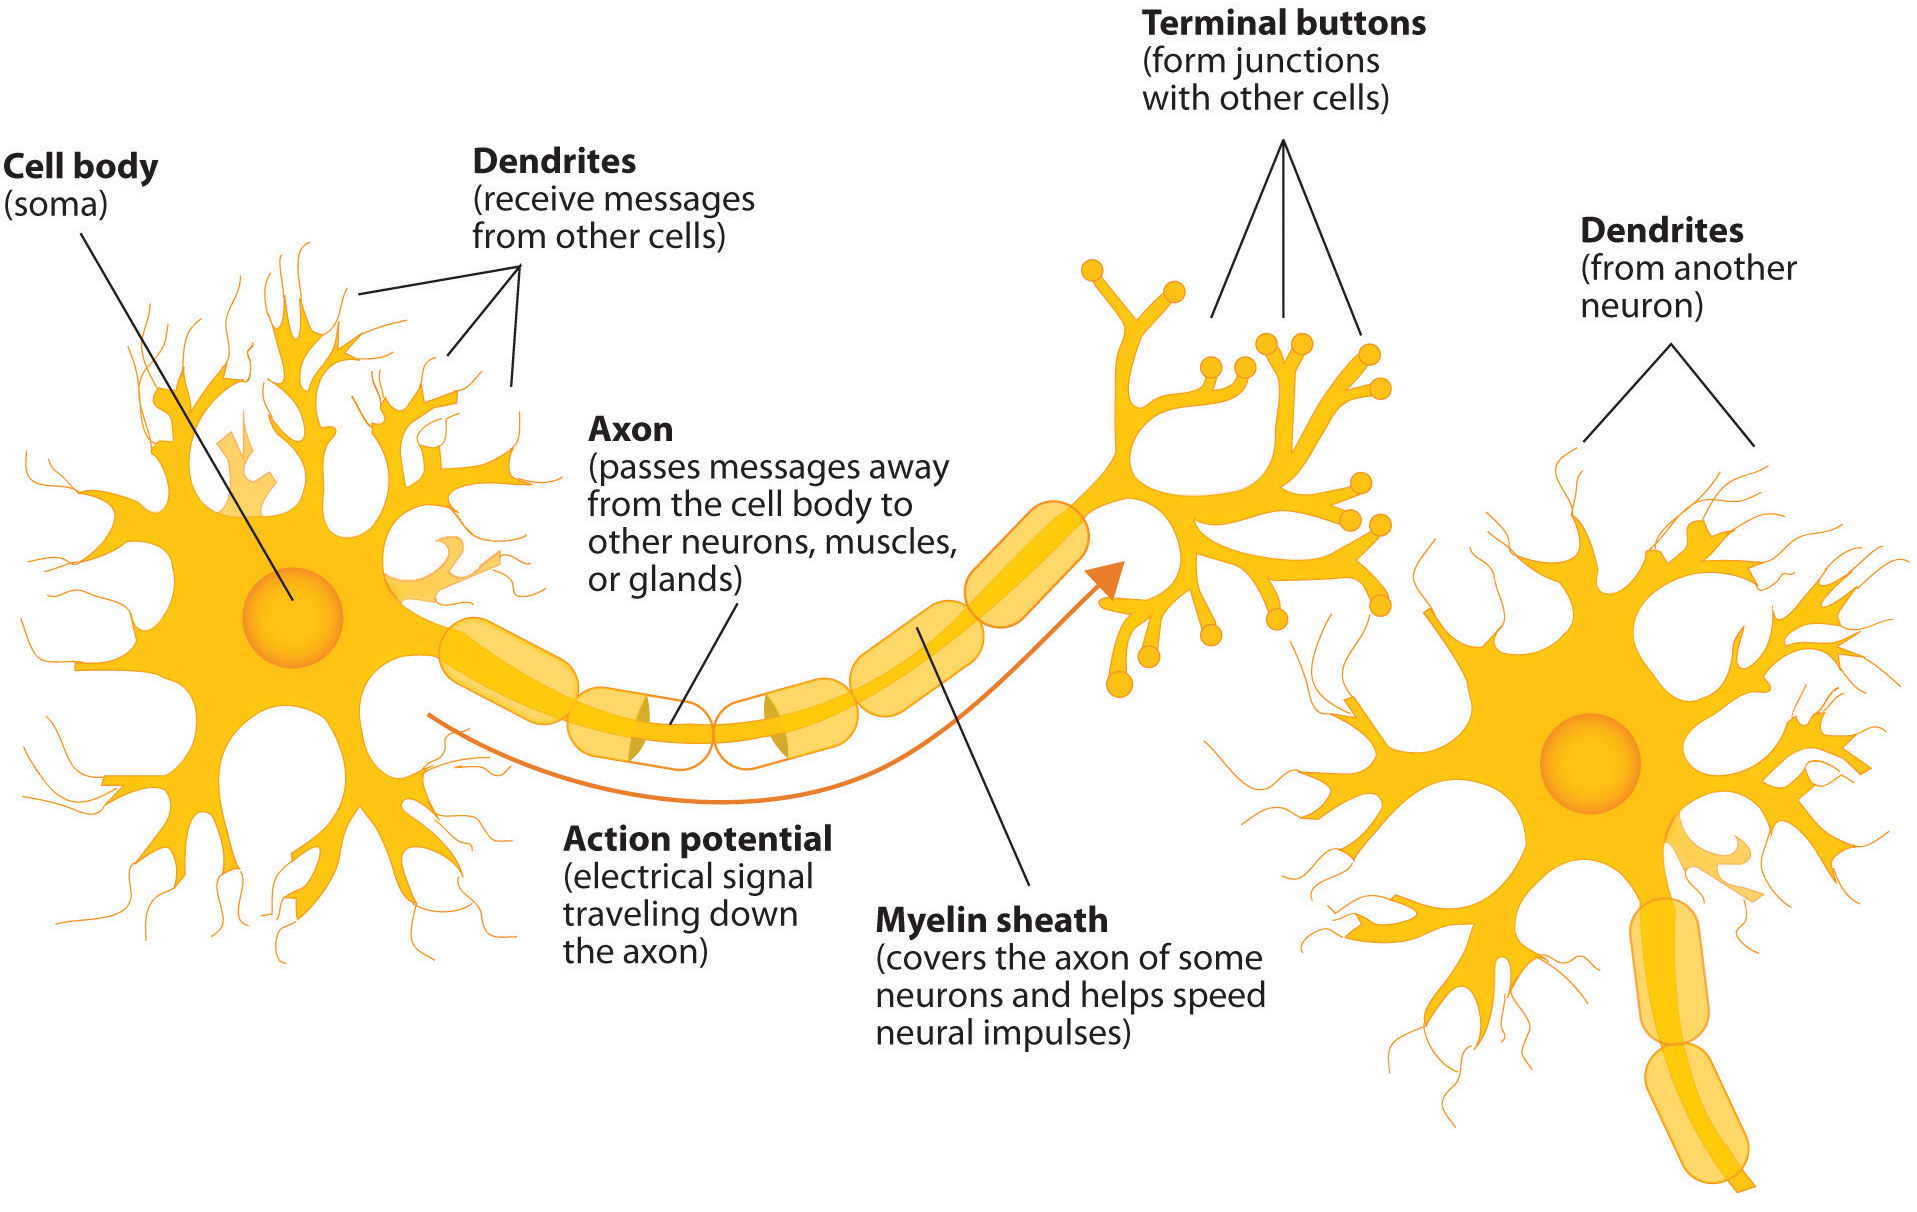
\includegraphics[width=0.99\textwidth]{components_of_neuron}
    \caption[Diagram of the components of a biological neuron]{A diagram of the components of a biological neuron. The image is from \citeay{wikipedia_neuron_2023}.}
    \figlbl{components_neuron}
\end{figure}

A biological neuron is a cell that communicates with other neurons through precisely timed electrical pulses called spikes or action potential.
Biological neurons are electrically excitable by voltage changes across their membranes.
The neuron generates an action potential if the changes are significant enough within a short interval.
This action potential propagates along the axon to the terminal buttons, activating synaptic connections to the dendrites of other neurons.
These components of a neuron are illustrated in \figref{components_neuron}.
The synaptic signal can be excitatory \sidecite{takagi_roles_2000} or inhibitory \sidecite{coombs_specific_1955}, making the postsynaptic neuron more or less likely to fire an action potential itself.
However, biological neurons do not follow strict rules; they adapt their firing rate to constant inputs, may continue firing after an input signal disappears and can even fire when no input is active \sidecite{wilson_spontaneous_1981, diamond_identifying_2019}.

Biological neurons can be classified into sensory neurons, motor neurons, and interneurons.
Sensory neurons respond to external stimuli such as light or sound and send signals to the spinal cord or the brain.
Motor neurons receive brain and spinal cord signals to control muscles or organs.
Interneurons establish connections between neurons within the same brain or spinal cord region.
However, this classification is a simplification, as the human brain consists of approximately 100 billion neurons \sidecite{herculano-houzel_human_2009} with diverse molecular, morphological, connectional, and functional properties \sidecite{zeng_neuronal_2017}.

Inspired by biological neurons, several variants of artificial neurons \sidecite{mcculloch_logical_1943, rosenblatt_perceptron_1958, fukushima_visual_1969} have been proposed in the literature and are discussed in \secref{ann}.
However, unlike their biological counterparts, artificial neurons are simplified models, ignoring much complexity. Like biological neurons, artificial neurons are usually connected to other neurons and form an artificial neural network \sidecite{prince_understanding_2023}. Although the neurons in the first layer of an artificial network could be considered sensory neurons, the neurons in the last layer could be considered motor neurons, and the neurons in the middle layer could be considered interneurons, this distinction is less meaningful because artificial neurons always have the same inner structure regardless of their position \sidecite{goodfellow_deep_2016}, except for variations in their activation function \cite{fukushima_visual_1969}.

Furthermore, artificial neural networks (ANNs) have a simpler organisational structure than the human brain. ANNs typically consist of one or a few network parts, such as encoders, which map data to a latent space, and decoders, which convert data from the latent space into a target vector \sidecite{goodfellow_deep_2016}. ANNs are considered monolithic because they are hierarchical and typically trained in an end-to-end fashion with a single error correction signal \sidecite{glasmachers_limits_2017}. In contrast, the human brain consists of many interconnected organisational units, each responsible for a specific function \sidecite{felleman_distributed_1991}. For example, in the cerebral cortex, which is responsible for vision, numerous small sub-units exist dedicated to specific tasks as illustrated in \figref{visual_cortext}.
Furthermore, the human brain does not comprise an organisational hierarchy as ANNs \sidecite{mountcastle_organizing_1978, mountcastle_columnar_1997}. In the human brain, each unit applies similar deterministic functions to the information it receives \cite{mountcastle_organizing_1978, mountcastle_columnar_1997}. Furthermore, the biological network in the human brain is dynamic and subject to change through growth and reorganisation, known as neuroplasticity or neuronal plasticity \sidecite{costandi_neuroplasticity_2016}.

In addition to the structural and functional differences, biological and artificial networks differ in their learning strategies.
An artificial learning system requires a feedback signal from which it can learn.
This is called the \emph{credit assignment problem}.
Backpropagation of error \sidecite{rosenblatt_principles_1962, linnainmaa_taylor_1976} is the state-of-the-art algorithm that solves this problem by propagating the error signals back through the network \sidecite{rumelhart_learning_1986}.
However, information in the brain flows only in one direction, from presynaptic to postsynaptic neurons.
Therefore, backpropagation of error is not biologically plausible \sidecite{grossberg_competitive_1987, crick_recent_1989}.
Furthermore, the brain relies on localised learning \sidecite{lillicrap_backpropagation_2020}, where each unit adapts its behaviour based on the information it receives.
Evidence suggests that the brain learns by connecting cells that are active at the same, which can be implemented with the Hebbian learning algorithm \sidecite{hebb_organization_1949}.
Researching biologically more plausible learning algorithms for artificial neural networks is a hot research topic summarised in \secref{alt_train_algo}.

\begin{figure}[h]
    \centering
    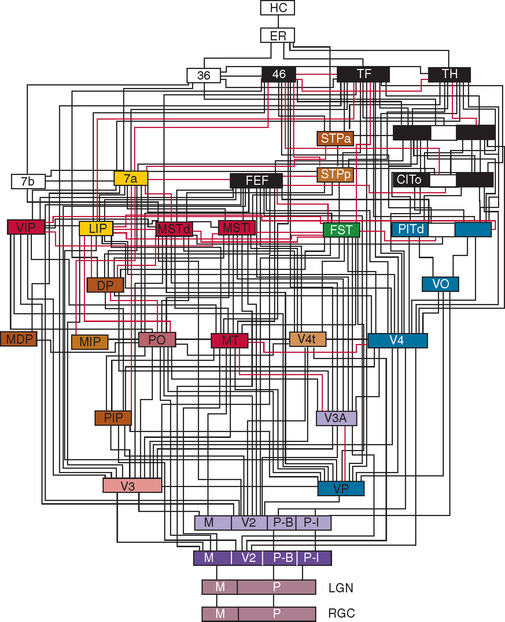
\includegraphics[width=0.89\textwidth]{felleman_visual_cortex}
    \caption[Organisation of the visual system in the cerebral cortex]{The organisation of the visual system in the cerebral cortex. The image is from \citeay{felleman_distributed_1991}.}
    \figlbl{visual_cortext}
\end{figure}

Thus, among the most important differences between biological and artificial neurons is the time-dependent and asynchronous firing of biological neurons compared to the synchronous firing of artificial neurons. In addition, biological networks have different types of neurons and rely on local learning, while artificial networks usually comprise identical neurons and utilise a global error correction algorithm. Finally, biological networks are organised in a complex way \sidecite{felleman_distributed_1991}, while artificial networks are composed of simpler connection patterns \sidecite{goodfellow_deep_2016}.

Biological findings strongly inspire the proposed vision framework.
Since biological systems still have many advantages compared to their artificial counterpart, the differences between these systems are of interest and could be promising in developing novel architectures.
Therefore, in \secref{neuroscience_findings}, biological principles related to the human's vision system are examined in more detail.

\section{Artificial Neural Networks}\seclbl{ann}
McCulloch and Pitts \sidecite{mcculloch_logical_1943} proposed the first model of a neuron that can be connected to other neurons.
Like the biological neuron, the artificial neuron of McCulloch and Pitts receives multiple input signals and transforms them into an output signal.
Their neuron takes a binary input vector $\boldsymbol{x} = (x_1, ..., x_n)$ where $x_i \in \{0, 1\}$ and maps it to an output $\hat{y} \in \{0, 1\}$.
The mapping from the input to the output is done by using an aggregation function $z = g(\boldsymbol{x})$ that sums up the input vector $\boldsymbol{x}$ and an activation function $f(z)$ that outputs $1$ if $z$ is bigger than a threshold $\theta$ and $0$ otherwise:
%
\begin{align}\eqlbl{McCulloch_Pitts_agg}%
	z &= g(\boldsymbol{x}) = g(x_1, ..., x_n) = \sum_{i=1}^{n}x_i\\
		\hat{y} &= f(z) = \begin{cases}
      		1, & \text{if}\ z \geq \theta \\
      		0, & \text{otherwise}
    	\end{cases}
\end{align}
%
The formula is often rewritten by using a bias $b$ instead of the  threshold $\theta$:
%
\begin{align}\eqlbl{McCulloch_Pitts_agg2}%
	z &= g(\boldsymbol{x}) = g(x_1, ..., x_n) = \sum_{i=1}^{n}x_i + b\\
		\hat{y} &= f(z) = \begin{cases}
      		1, & \text{if}\ z \geq 0 \\
      		0, & \text{otherwise}
    	\end{cases}
\end{align}
%
By adjusting the bias $b$, neurons can learn to fire under different conditions.
In 1958, \sideciteay{rosenblatt_perceptron_1958} proposed the perceptron, which extends the neuron with additional learnable weights: The input vector $\boldsymbol{x}$ of length $n$ is multiplied with a weight vector $\boldsymbol{w} \in \mathbb{R}^n$ of the same length.
%
\begin{align}\eqlbl{nn}%
	z = g(\boldsymbol{x}) = \boldsymbol{w} \cdot \boldsymbol{x} + b = \left( \sum_{i=1}^{n}w_i \cdot x_i \right) + b
\end{align}
%
The weight vector $\boldsymbol{w}$ remains identical if the output $\boldsymbol{\hat{y}}$ corresponds to the desired output $\boldsymbol{y}$ or is adjusted otherwise (c.f. \secref{learning_algorithm}). Later, the activation function \(f(z)\) was replaced with other functions so that the output can be a real number \(\hat{y} \in \mathbb{R}\) \sidecite{fukushima_visual_1969}. Often-used activation functions are
%
\begin{align}\eqlbl{act_functions}%
		\text{Sigmoid: } & f(z) = \sigma(z) = \frac{1}{1+\mathrm{e}^{-z}}\\
		\text{Rectified linear unit (ReLU): } & f(z) = (z)^{+} = \max\{0, z\}\\
		\text{Hyperbolic tangent (tanh): }  & f(z) = \tanh(z) = \frac{\mathrm{e}^{z}-\mathrm{e}^{-z}}{\mathrm{e}^{z}+\mathrm{e}^{-z}}
\end{align}


To summarise, artificial neurons multiply incoming signals with learned weights and add a bias before applying a non-linear activation function.
Unlike their biological counterparts, artificial neurons exhibit non-temporal behaviour and output continuous values instead of discrete binary spikes. Neurons with time-dependent spike patterns are discussed in \secref{spiking_networks}.

\subsection{Fully Connected Layer}\seclbl{fully_connected_layer}
Artificial neural networks (ANNs) consist of several neurons organised in a network. These neurons are arranged in layers \cite{prince_understanding_2023}. In a basic configuration, each neuron in one layer is connected to each neuron in the following layer, forming a so-called fully connected layer (FC) \sidecite{prince_understanding_2023, goodfellow_deep_2016}.

In a fully connected layer with $k$ neurons, the input $\boldsymbol{x} \in \mathbb{R}^n$ is multiplied with a weight matrix $\boldsymbol{W} \in \mathbb{R}^{n\times k}$ and a bias $\boldsymbol{b} \in \mathbb{R}^k$ is added to obtain the layer's output $\boldsymbol{\hat{y}} \in \mathbb{R}^k$:
\begin{align}\eqlbl{nn3}%
	\boldsymbol{z} = \boldsymbol{W} \cdot \boldsymbol{x} + \boldsymbol{b}
\end{align}
\begin{align}
	\hat{\boldsymbol{y}} = f(\boldsymbol{z})
\end{align}
%
The universal approximation theorem \sidecite{cybenko_approximation_1989} states that a shallow network with one hidden layer (i.e. one layer between input and output layer) and enough neurons can approximate any mapping function between inputs and outputs.
However, a sequential arrangement of multiple layers is more efficient for complex functions \sidecite{prince_understanding_2023}. This hierarchical approach allows the network to learn a hierarchy of features and capture intricate patterns \sidecite{bengio_deep_2012}.

In a multi-layer perceptron (MLP) with $L$ layers, the input \(\boldsymbol{x}\) is passed through each layer, whereby each subsequent layer \(l\) uses the output of the previous layer \(l-1\) as input.
The layers in the network are denoted with a superscript square bracket notation, where $l$ is the layer index. 
For instance, the weights of layer $l$ are denoted as $\boldsymbol{W}^{[l]}$, the bias as \(\boldsymbol{b}^{[l]}\), the output of the aggregation function as \(\boldsymbol{z}^{[l]}\), and the output of the activation function as \(\boldsymbol{a}^{[l]}\).
The input in the first layer is the input data itself, i.e. $\boldsymbol{a}^{[0]} = \boldsymbol{x}$, and the output of the last layer corresponds to the model's prediction, denoted as $\boldsymbol{a}^{[L]} = \hat{\boldsymbol{y}}$. With this notation, the mathematical formulation of an MLP can be defined as follows:
%
\begin{align}\eqlbl{mlp}
		\boldsymbol{z}^{[l]} = \boldsymbol{W}^{[l]}\boldsymbol{a}^{[l-1]} + \boldsymbol{b}^{[l]}
\end{align}
%
\begin{align}\eqlbl{mlp2}
		\boldsymbol{a}^{[l]} = f(\boldsymbol{z}^{[l]})
\end{align}

A significant drawback of this approach is, as outlined in \secref{intro_motivation}, that layer-wise data processing leads to early commitment \sidecite{marr_vision_2010}.
The problem is that the first layers already commit to representations and steer the learning process in specific directions without considering higher-level features.
The framework proposed in this thesis introduces a novel layer that builds hierarchical representations within the same layer (c.f. \secref{framework_building_blocks}), efficiently preventing the fallacy of early commitment.


\subsection{Convolutional Networks}\seclbl{cnns}
A problem of fully connected layers is that they are not position invariant, meaning they cannot recognise patterns regardless of their location in the input.
Convolutional neural networks (CNNs) \sidecite{fukushima_neocognitron_1980, waibel_phoneme_1987, lecun_backpropagation_1989} are inspired by biological processes \sidecite{fukushima_visual_1969, hubel_receptive_1968} and can overcome this limitation: CNNs exhibit position equivariance by applying the same weights at all input positions \cite{gerber_stride_2020}.
A typical CNN consists of subsequently connected convolutional layers and pooling layers.
Usually, an activation function is applied after each convolutional layer, while no activation function is used after pooling layers \cite{goodfellow_deep_2016}.

Convolutional layers employ convolution filters or kernels that slide along the input, generating translation-equivariant \cite{gerber_stride_2020} responses known as feature maps \cite{zhang_parallel_1990}.
Translation-equivariant means that the relative placement of objects remains consistent between the layer's input and output, as the same filter is applied to all image positions.
During the filtering process, the dot product is calculated between the filter and an input area (of the same size as the filter), resulting in a scalar value that is assigned to one position of the output matrix (i.e. the feature map) \sidecite{goodfellow_deep_2016}.
This process is repeated by shifting the filter by a specified stride until the entire input is processed and all values in the output matrix are calculated.
Convolutional layers require much fewer parameters than fully connected layers of the same size because only the kernels need to be learned.
This process of reusing the same weights at different input locations is known as parameter sharing \sidecite{gerber_stride_2020}.
By stacking multiple layers, CNNs become hierarchical: The convolutional operation squeezes information from surrounding pixels into a single output cell. Thus, using multiple layers sequentially continuously enlarges the receptive field - the area of input pixels that can influence a single value in a layer's feature map \sidecite{bengio_deep_2012}.

Pooling layers downsize the input rather than extracting features \sidecite{ciresan_flexible_2011}.
Similar to convolutional layers, they slide a filter along the input.
However, unlike convolutional layers, pooling filters do not have learned parameters but use an aggregation function.
Usually, the filter selects the pixel with the highest value (max pooling) or calculates the average (average pooling) within the considered input area and uses this value as output \cite{ciresan_flexible_2011}.
The filter is then shifted by its size, ensuring that non-overlapping image patches are processed.
Pooling layers discard a considerable amount of information but effectively reduce complexity and improve the model's robustness \cite{ciresan_flexible_2011}.
Discarding valuable information can also be the reason for misclassification \sidecite{sharma_implications_2019}.

Besides CNNs, alternative architectures for image processing have emerged that are characterised by position invariance, such as the vision transformer (ViT) \sidecite{dosovitskiy_image_2021} or MLP mixer \sidecite{tolstikhin_mlp-mixer_2021}. However, providing an in-depth description of these architectures would exceed the scope of this introduction to deep learning.

\subsection{Learning Algorithm}\seclbl{learning_algorithm}
The model's prediction $\boldsymbol{\hat{y}}$ will only be close to the target output $\boldsymbol{y}$ if the weights $\boldsymbol{W}^{[l]}$ and biases $\boldsymbol{b}^{[l]}$ are properly defined.
These parameters are learned through training, typically using backpropagation of errors \sidecite{rosenblatt_principles_1962, linnainmaa_taylor_1976}.
Training can take place in a supervised, unsupervised, semi-supervised or reinforcement learning setting \sidecite{russell_artificial_2021, simmler_survey_2021}. In supervised learning \sidecite{cord_supervised_2008}, the model output $\boldsymbol{\hat{y}}$ is compared to a target output $\boldsymbol{y}$. Self-supervised (also called unsupervised) learning \cite{liu_self-supervised_2021} finds patterns in input data without predefined labels. Typically, the target $\boldsymbol{y}$ is derived from the data automatically, for example, by predicting a masked part of the data \cite{radford_improving_2018}. Semi-supervised learning \cite{van_engelen_survey_2020} combines labelled and unlabelled data. Lastly, reinforcement learning algorithms \cite{arulkumaran_deep_2017} aim to maximise the rewards they receive from environments based on their actions.

All these learning principles have in common that a loss function \cite{wang_comprehensive_2022} (also called an objective function) $\mathcal{L}(\boldsymbol{\hat{y}}, \boldsymbol{y})$ is used to calculate the quality of the model output $\boldsymbol{\hat{y}}$ relative to the target output $\boldsymbol{y}$.
The selected loss function is minimised iteratively using an error correction algorithm such as stochastic gradient descent (SGD)\sidenote{There also exist other optimisation algorithms such as SGD with momentum, RMSprop or Adam \cite{kingma_adam_2017}.}. This process continues until the network reaches a (local) minimum.
Stochastic gradient descent is based on the insight that the negative gradient of the loss value indicates the direction of the steepest descent, i.e. the direction in which the loss decreases the most. Consequently, SGD updates the parameters of the network by taking steps of size $\eta$ (the learning rate) in the direction of the negative gradient:
%
\begin{align}\eqlbl{sgd}
	\begin{aligned}
		\Delta \boldsymbol{W}^{[l]} = & -\eta \cdot \left( \nabla_{\boldsymbol{W}^{[l]}} \mathcal{L}(\boldsymbol{\hat{y}}, \boldsymbol{y}) \right)\\
		\boldsymbol{W}^{[l]} \coloneqq & \boldsymbol{W}^{[l]} + \Delta \boldsymbol{W}^{[l]}
	\end{aligned}
\end{align}
%
and
%	
\begin{align}\eqlbl{sgd2}	
	\begin{aligned}
		\Delta \boldsymbol{b}^{[l]} = & -\eta \cdot \left( \nabla_{\boldsymbol{b}^{[l]}} \mathcal{L}(\boldsymbol{\hat{y}}, \boldsymbol{y}) \right)\\
		\boldsymbol{b}^{[l]} \coloneqq & \boldsymbol{b}^{[l]} + \Delta \boldsymbol{b}^{[l]}
	\end{aligned}
\end{align}
%
The term $\left( \nabla_{\boldsymbol{W}^{[l]}} \mathcal{L}(\boldsymbol{\hat{y}}, \boldsymbol{y}) \right)$ is the gradient of the weights $\boldsymbol{W}^{[l]}$  with respect to the loss $\mathcal{L}(\boldsymbol{\hat{y}}, \boldsymbol{y})$ and the term $\left( \nabla_{\boldsymbol{b}^{[l]}} \mathcal{L}(\boldsymbol{\hat{y}}, \boldsymbol{y}) \right)$ is the gradient of the bias \(\boldsymbol{b}^{[l]}\)  with respect to $\mathcal{L}(\boldsymbol{\hat{y}}, \boldsymbol{y})$.
The gradients of the weights can efficiently be calculated with backpropagation of error \sidecite{rosenblatt_principles_1962, linnainmaa_taylor_1976}, which is, in fact, just an intelligent implementation of the chain rule\sidenote{While a detailed discussion of backpropagation is out of scope for this thesis, we refer interested readers to the book ``Understanding Deep Learning'' by \citeay{prince_understanding_2023}.}.

Using a global error correction algorithm such as backpropagation of error optimises consistency between the prediction $\boldsymbol{\hat{y}}$ and the teaching signal $\boldsymbol{y}$.
This works well for specific tasks \sidecite{bertolini_machine_2021, zou_object_2023}.
In contrast, the human brain optimises consistency between each cell utilising a local learning principle \sidecite{hebb_organization_1949}. 
As outlined in \secref{intro_motivation}, local learning and optimising consistency between all cells prevents early commitment \sidecite{marr_vision_2010}, a fundamental principle in the biological vision system \sidecite{von_der_malsburg_theory_2022}.
Leveraging this principle, as done in this thesis, could help to overcome intrinsic issues of deep learning systems.

\section{Limitations}\seclbl{limitationsDL}
Deep learning systems have proven themselves as excellent feature extractors and are used to fulfil various tasks in our daily lives.
Nevertheless, they have several limitations, with some of the most pressing ones elucidated below.

\paragraph{Computing Resources.} Deep learning models are typically trained on modern computing infrastructure. They benefit from Moore's law \sidecite{moore_cramming_1965}, stating that the number of transistors in a dense integrated circuit doubles every two years, allowing models to consume exponentially more computing resources. However, the physical limits of transistor size will most likely stop this exponential growth soon \sidecite{kumar_fundamental_2015}, and the future progress of hardware remains uncertain.
Furthermore, the size of modern deep learning models exhibits an even faster growth, as demonstrated by state-of-the-art large language models: 
ELMo from 2018 uses around 94 million parameters \sidecite{peters_deep_2018}, 
GPT-3 from 2020 uses around 175 billion parameters \sidecite{brown_language_2020}, and Megatron-Turing NLG from 2022 has 530 billion parameters \cite{smith_using_2022}.
An analysis by \citeay{open_ai_ai_2018} shows exponential growth in computational usage by AI models, with a doubling time of about 3.4 months, outpacing the rate of hardware progress, which has a doubling time of 2 years. Moreover, the increasing size of deep networks poses a challenge for inference on low-budget hardware such as smartphones or embedded systems \sidecite{berthelier_deep_2021}. Although techniques such as quantisation \sidecite{wu_integer_2020}, model pruning \sidecite{choudhary_comprehensive_2020} and model distillation \sidecite{zhou_distilling_2021} exist to reduce model size after training, the question is whether increasing model size is the best way to develop more advanced systems regarding feasibility but also regarding energy consumption \sidecite{garcia-martin_estimation_2019}.

\paragraph{Catastrophic Forgetting.} Another major issue of deep learning systems is that they suffer from catastrophic forgetting \sidecite{kirkpatrick_overcoming_2017, liu_overcoming_2021}.
If a model is trained on a specific task and afterwards trained (or fine-tuned) on another task, the model suffers a ``catastrophic'' drop in performance over the first task \cite{kirkpatrick_overcoming_2017}.
The reason for this effect is that during training on the second task, the model adjusts the parameters learned during the first task and, therefore, ``forgets'' the learned input-output mapping functions.
Mixing all datasets or learning all tasks in parallel in a multi-task setting \sidecite{zhang_survey_2022} does not seem feasible to prevent catastrophic forgetting. Instead, models should remember previously learned knowledge even if a new task is learned.
Online learning \sidecite{sahoo_online_2018} and lifelong learning \sidecite{parisi_continual_2019} do not solve catastrophic forgetting as they only allow models to adapt better to changing conditions.

\paragraph{Extrapolate Data Distribution.} It is questionable if deep learning models can achieve \emph{real} generalization\sidenote{Generalisation refers to the ability of the model to adapt appropriately to previously unseen data from the same distribution.} in the current learning framework.
With enough data, deep learning can achieve generalisation in the sense that the model can interpolate within the known data distribution.
However, deep learning models fail to extrapolate.
For example, convolutional neural networks (CNNs) do not generalise to different viewpoints unless added to the training data \sidecite{madan_when_2022}.
%The reason is that the networks are optimised to learn a model of observed data and typically have a high degree of freedom (i.e. many parameters).
%Thereby, they tend to learn (too) complex models of the data: For example, modern language models have up to 530B neurons to fulfil a single task \cite{smith_using_2022}, while the human brain has 100B binary neurons in total \cite{herculano-houzel_human_2009}.
%Furthermore, such artificial networks do not reason about the learned model. For example, humans believed for thousands of years in the geocentric model (the earth is in the centre of the universe) until the heliocentric model (the sun is in the centre) superseded it. Artificial networks lack this ability to reason about the best model for observed data. Instead, they tend to make minor adjustments to the existing model until it no longer improves.

\paragraph{Data Hunger.} Deep learning cannot learn abstract relationships in a few trials but requires many samples and is thus data-hungry.
Gary Marcus \sidecite{marcus_deep_2018} showcased this problem with an example: He defines the new word ``schmister'' as a sister over the age of 10 but under the age of 21. He found that humans can immediately infer whether they or their best friends have any ``schmister''. However, modern deep learning systems lack a mechanism for learning abstractions through explicit, verbal definitions and require thousands or even more training samples\sidenote{LLMs can deal with such definitions when they are put into the context during inference but not when the example is only shown once during training.}.

\paragraph{Casual Reasoning.} No deep learning model has been able to demonstrate causal reasoning generically.
Deep learning models find correlations between input and output data but not causation \sidecite{prince_understanding_2023}.
Other AI approaches, such as hierarchical Bayesian computing \cite{allenby_hierarchical_2005} or probabilistic graphical models \cite{koller_probabilistic_2009} are better at causal reasoning but do not work well for processing high-dimensional data.

\paragraph{Embodiment.} Deep learning models are, to some extent, too isolated since they have no embodiment and cannot interact with the world.
For example, the human body provides needs, goals, emotions, and gut feelings \sidecite{mayer_gut_2011}. One could argue that the body is, therefore, a co-processor of the brain.
In current deep learning systems, emotions are absent, and the goals are set externally \sidecite{wang_comprehensive_2022}.
Deep reinforcement learning \sidecite{dong_deep_2020} is a first step toward dissolving this isolation as the models interact with a virtual environment. 
However, AI systems interacting with the real world have not worked well so far.
Moravec's paradox from 1995 \sidecite{moravec_mind_1995} states that ``it is comparatively easy to make computers exhibit adult level performance on intelligence tests or playing checkers, and difficult or impossible to give them the skills of a one-year-old when it comes to perception and mobility''.
This statement still seems true almost $30$ years later.

These drawbacks are likely due to statistical learning based on a global error correction algorithm.
In contrast, the human brain does not suffer from these drawbacks, indicating that different learning principles could resolve these issues.
The framework proposed in this thesis introduces new learning principles that aim to reduce computational requirements, catastrophic forgetting, and data hunger and allow better data extrapolation as outlined in \secref{discussion}.


\section{Neurocomputing}\seclbl{neurocomputing}
Neurocomputing is a subfield of neuroscience that focuses on implementing learning algorithms that adhere to biological plausibility. Thus, researchers are addressing the discrepancy described in \secref{neurons} and striving to develop alternative learning principles.

\subsection{Hebbian Learning}\seclbl{hebbian}
Hebbian learning, as proposed by \sideciteay{hebb_organization_1949}, implements the adaptive nature of the connections between cells in the nervous system. Hebb's description states that when an axon of cell $A$ is in close proximity to cell $B$ and consistently contributes to its firing, growth processes or metabolic changes occur in one or both cells that increase the effectiveness of cell $A$ in firing cell $B$. This description is often summarised as ``neurons that fire together wire together''.

Hebbian learning describes the update of the synaptic weight $w_{ij}$ connecting neuron $i$ to neuron $j$ according to the aforementioned principles. The weight change depends on the presynaptic activity $a_i$ of neuron $i$ and postsynaptic activity $a_j$ of neuron $j$\sidenote{The presynaptic and postsynaptic activity corresponds to the output of a neuron's activation function $f(\cdot)$ in the preceding and subsequent layers.}:
%
\begin{align}\eqlbl{hebb_1}
	\Delta w_{ij} = \eta a_i a_j
\end{align}
%
where \(\eta\) is the learning rate.
Hebbian learning is used in the proposed framework to increase the weights between frequently co-activated binary neurons (c.f. \secref{framework_hebb_updates}).
This rule causes two cells that are constantly active together to form an ``association'' where the activation of one cell promotes the activation of the other.
Therefore, a network trained according to Hebb's rule is able to ``auto-associate'' a pattern \cite{hebb_organization_1949}. In other words: When the pattern is activated, cells associated with that pattern are also activated, while cells not associated with the dominant pattern are inhibited. These learned patterns are called engrams \sidecite{newman_current_1985}, often related to memories in a biological context \sidecite{liu_optogenetic_2012}.

The aforementioned Hebbian rule increases the weight between two binary cells that are active together and does not change when only one or none of the cells fires. Thus, the connection can only grow stronger.
However, synapses can not only grow between cells but also disintegrate \sidecite{costandi_neuroplasticity_2016}.
This process can be implemented by leveraging the covariance of neuronal activity \sidecite{oja_simplified_1982}.
The covariance is positive if two neurons fire often together and negative if they do not often fire together.
The following equation changes the weight relative to the covariance:
%
\begin{align}\eqlbl{hebb_2}
	\Delta w_{ij} = \eta (a_i - \psi_i) \cdot (a_j - \psi_j)
\end{align}
%
where \(\psi_i\) and \(\psi_j\) are estimates of the expected pre- and postsynaptic activity\sidenote{The expected activity can be estimated, for example, by calculating a moving average.}.

The formula above lacks two important constraints.
First, the weight growth has no upper or lower bound: With long training on the same patterns, a synaptic connection $w_{ij}$ constantly increases or decreases. In practice, boundaries are defined to mitigate this issue. This can be implemented by normalising the length of the weight vector \cite{oja_simplified_1982} or by using rate-based threshold adaption \sidecite{bienenstock_theory_1982, intrator_objective_1992}.
Second, breaking the symmetry within the network is necessary: After initialisation, many cells tend to fire simultaneously, resulting in many similar updates of the synaptic connections. However, independent neurons can encode more information and work better than dependent neurons \sidecite{simoncelli_natural_2001}.
Thus, competition between neurons is needed to encourage differentiation, allowing only a subset of connections to be updated.
Well-known approaches are winner-take-all competition, using a recurrent circuit that provides a competitive signal, anti-Hebbian learning \sidecite{vogels_inhibitory_2011} (a method that adds a penalty for similarly active neurons), or adapting the activation function of the neurons to enforce a specific activity distribution \sidecite{joshi_rules_2009, teichmann_intrinsic_2015}.

Hebbian learning can be considered an alternative to backpropagation of error \cite{rosenblatt_principles_1962, linnainmaa_taylor_1976}.
Hebbian learning does not propagate error signals backwards but relies on a self-organisation process.
In this thesis, Hebbian learning is leveraged as it allows to prevent early commitment, even though self-organising processes are more complex to train than global error correction algorithms \sidecite{risi_future_2021}.


\subsection{Hopfield Networks}\seclbl{hopfield}
The Hebbian rule can be used to train Hopfield networks.
Hopfield networks serve as associative (i.e. content-addressable) memory systems \sidecite{hopfield_neural_1982}, similar to the nearest neighbour algorithm \sidecite{fix_discriminatory_1989} or memory networks \cite{weston_memory_2015}.
In a Hopfield network, all neurons are connected without self-connections, i.e. $w_{ii}=0$.
Additionally, the synaptic weights in a Hopfield network are symmetrical, meaning \(w_{ij} = w_{ji}\).
In the subsequent discussion, these networks will be referred to as binary Hopfield networks, as they operate exclusively with binary units.

An input is fed into the network by setting the neuronal activity $\boldsymbol{a}[t=0]$ at time $t=0$ to a specific configuration.
Hopfield networks have temporal dynamics, and the output evolves over time: After the initial input is set as the network's state, the cells influence each other, and the network's state is updated until a stable attractor state is reached.

The state of a neuron at time $t+1$ depends on the state of all other neurons at time $t$ within the network:
%
\begin{align}\eqlbl{hf_1}
	z_i[t+1] = \sum_{i \neq j} w_{ij} a_j[t] + b_i
\end{align}
%
\begin{align}\eqlbl{hf_2}
	a_i[t+1] = \begin{cases}
      		1, & \text{if } z_i[t+1] > 0 \\
      		-1, & \text{otherwise}
    	\end{cases}
\end{align}
%
When the aggregation value $z_i$ is bigger than $0$, the cell turns on or turns off otherwise.
Thus, a cell can either keep its state ($a_i[t+1] = a_i[t]$) or flip ($a_i[t+1] \neq a_i[t]$).
A flipping state influences all other neurons and may encourage them to flip as well.
There exists formal proof that after a finite number of timesteps, an attractor state is reached, and the neurons do not flip anymore \sidecite{hopfield_neural_1982}.
An input pattern is attracted to the closest stable pattern.
Hebbian learning (c.f. \secref{hebbian}) can be used to define what the stable patterns are:
With a single iteration over the training patterns, the weights $w_{ij}$ and biases $b_i$ are updated so that these patterns become attractor states \sidecite{hopfield_unlearning_1983}.
This allows using the network as an associative memory, i.e. to map an input pattern to the most similar predefined stable pattern.

For a long time, Hopfield networks had two limiting factors: First, the capacity $C$, i.e. the number of patterns that can be stored, was for a network with $k$ neurons limited to $C=0.138k$ \sidecite{mceliece_capacity_1987}.
However, this limitation could be resolved more than three decades after the introduction of the binary Hopfield networks; 
\sideciteay{krotov_dense_2016} first increased the capacity to a polynomial capacity w.r.t. $k$ and \sideciteay{demircigil_model_2017} later to exponential capacity w.r.t. $k$.
The second limiting factor of binary Hopfield networks is that only binary patterns can be stored.
Recently, Hopfield networks have been extended to continuous patterns \sidecite{ramsauer_hopfield_2021}.
Continuous Hopfield networks can retrieve continuous patterns or a combination of several similar continuous patterns.

Currently, Hopfield networks remain a niche, as they perform worse than retrieval systems \sidecite{kowalski_information_1997} and memory networks \sidecite{weston_memory_2015}.
They also lack hierarchical pattern recognition and may require additional models to store higher-level patterns than just the input data.
In the context of the proposed framework, a Hopfield network could be used as a biologically plausible memory, storing concrete instances of objects.
However, such a memory is not investigated within the context of this thesis and remains an open question for future research.


\subsection{Spiking Neural Networks}\seclbl{spiking_networks}
Biological neurons emit time-dependent spikes (c.f. \secref{neurons}).
To transmit information, especially the firing rate (i.e. the number of spikes per second) and precise timing of the spikes are relevant \sidecite{eckmiller_spike_1990}.
The amplitude and duration of the spike matter less.
So-called spiking neural networks (SNNs) incorporate the concept of time into a computational model \sidecite{maass_networks_1997}.
SNNs do not transmit information in each forward pass but rather send a signal when the membrane potential reaches a threshold value\sidenote{The membrane potential is related to the electrical charge of the membrane of a biological neuron.}. 
The most prominent models of spiking neurons are different integrate-and-fire (IF) neurons \sidecite{abbott_lapicques_1999, izhikevich_simple_2003, brette_adaptive_2005}.
While each model has different mathematical properties, the concept remains the same: Each neuron has a membrane potential that is increased or decreased through spikes from other neurons and decays over time or is reset when the cell emits a spike.

The synaptic plasticity can be learned with an adapted version of Hebbian learning, called the spike-timing-dependent (STDP) plasticity rule \sidecite{bi_synaptic_2001}.
This rule strengthens connections if the presynaptic neurons fire before the postsynaptic neuron and weakens the connection otherwise.

For a long time, SNN only worked for very shallow networks.
In 2018, \sideciteay{kheradpisheh_stdp-based_2018} proposed a deep spiking convolutional network inspired by CNNs to overcome this limitation.
This network uses convolutional and pooling layers with IF neurons traditional of classical artificial neurons and is trained with STDP.
Despite these remarkable advances in SNNs, their performance is still inferior compared to equivalent artificial neural networks \sidecite{nunes_spiking_2022}. Several factors contribute to this discrepancy. First, SNNs require converting inputs, such as images, into spike representations.
However, this process results in losing important information, including colour and texture details. In addition, SNNs use non-differentiable activation functions, which makes them unsuitable for training by backpropagation of error. Consequently, alternative training strategies must be developed to achieve similar benchmark scores as ANNs \cite{nunes_spiking_2022}.

Even though spiking neurons are biologically more plausible than neurons without time dependency, they are not used in the proposed framework.
The reasons are that they do not provide an obvious advantage despite their plausibility and do not seem very suitable for processing a static input (e.g. an image) on a clocked machine (e.g. a CPU).

%\subsection{Reservoir Computing}\seclbl{reservoir_comp}
%Reservoir computing is an umbrella term for networks based on the concepts of echo-state networks (ESN) \sidecite{jager_echo_2001} and liquid-state machines (LSM) \sidecite{maass_real-time_2002}.
%ESNs use perceptrons as a model of neurons, while LSMs are based on spiking neurons (c.f. \secref{spiking_networks}).
%These networks belong to the broader field of recurrent neural networks (RNNs) \cite{} and are designed to handle time-dependent or sequential data efficiently.

%In traditional RNNs, the entire network, including input, hidden and output layers, is trained together to learn temporal dependencies. This training process can be computationally intensive and time-consuming. Reservoir computing takes a different approach: It consists of a reservoir and a linear readout layer, whereby only the readout layer requires iterative training.
%Thus, a key advantage of such systems is that the reservoir dynamics are fixed, and only the readout stage is trained.

%The reservoir is an untrained, randomly connected network of recurrent cells. The connections are fixed, but the recurrent cells encourage rich internal dynamics \sidecite{tanaka_recent_2019}. When an input sequence is fed into the reservoir, the dynamics of the reservoir transform the input into a high-dimensional representation in its state space. This transformation is achieved by passing the input through the recurrent connections of the reservoir.
%A good reservoir system distributes different inputs into different regions of the computation space \sidecite{adamatzky_reservoir_2018}.

%After the reservoir has processed the input, a linear readout layer maps the reservoir's state to the desired output. The readout layer usually consists of a linear regression model or a single-layer neural network \cite{tanaka_recent_2019}. Since the reservoir already encodes the temporal information from the input sequence, the task of the readout layer is simplified as it only needs to perform a linear mapping of the reservoir state to the desired output.
%
%\begin{figure}[h]
%    \centering
%    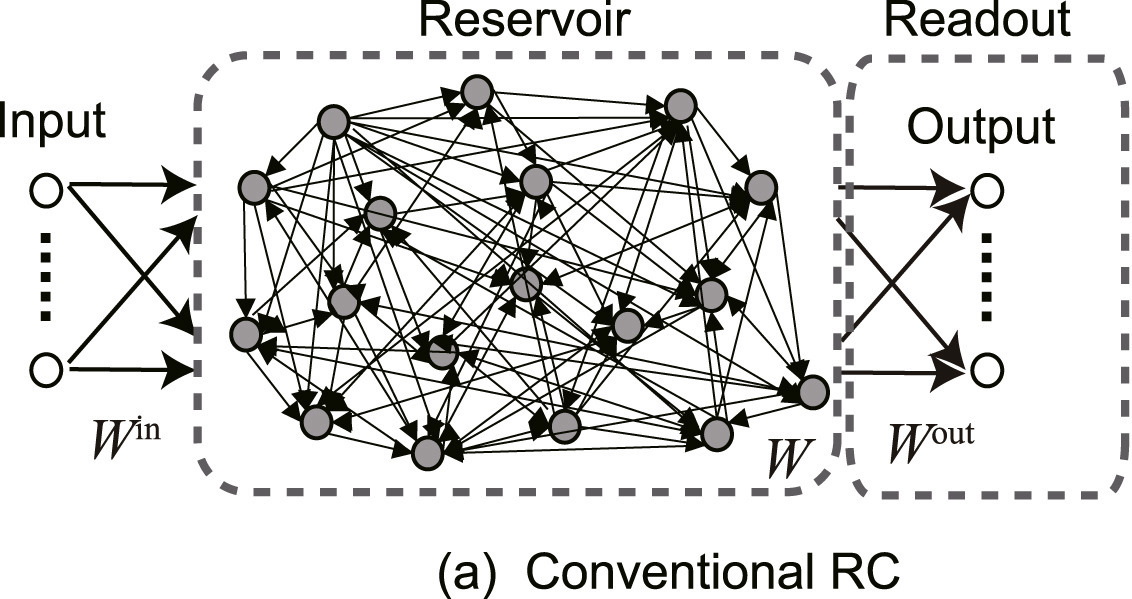
\includegraphics[width=0.79\textwidth]{reservoir}
%    \caption[Structure of an echo state network]{Structure of an echo state network. The image is from \citeay{tanaka_recent_2019}.}
%    \figlbl{reservoir}
%\end{figure}
%
%The main distinction between reservoir computing frameworks lies in reservoir design.
%An ESN uses the perceptron as the model of neurons and connects them with recurrent connections according to an Erdős–Rényi graph model\sidenote{The Erdős–Rényi model is a model for generating random graphs where all graphs based on a fixed set of vertices and edges are equally likely.} \sidecite{erdos_random_1959}.
%LSM, on the other hand, use a spiking neural network instead of a graph of recurrent cells.
%The nodes of the spiking neural network are randomly connected.
%Thus, every node receives time-varying inputs from other nodes.

%The weights of the reservoir connections are randomly assigned and remain unchanged throughout the training process. The readout layer is trained with a supervised learning algorithm such as ridge regression or gradient descent to minimise the discrepancy between predicted and desired outputs.
%Thus, the training is very efficient and does not require complex training algorithms, while the system can still efficiently process temporal data.

%In general, reservoirs are universal approximators and can approximate any non-linear function, given that there are enough neurons in the reservoir.
%In principle, the system should be capable of any computation if it has a high enough complexity \cite{adamatzky_reservoir_2018}.
%Recently, reservoir computing has become popular in quantum computing \cite{ghosh_quantum_2019, chen_temporal_2020} and for chaotic signal processing \cite{vlachas_backpropagation_2020, krishnagopal_separation_2020}.
%However, they are still limited and can only deal well with low-dimensional temporal data. Furthermore, their performance is typically worse than comparable artificial neural networks on most benchmarks \cite{tanaka_recent_2019}.
